%%%%%%%%%%%%%%
% BASIC FORMATTING %
%%%%%%%%%%%%%%

\documentclass[11 pt]{article}
%\documentclass[10 pt]{amsart}

%LOAD VARIOUS PACKAGES
\usepackage{amsmath,amssymb,amsthm,amsfonts,graphicx,url,colordvi}
\usepackage{graphics,graphics,latexsym,multicol}
\usepackage{enumerate}

%SET MARGINS
\usepackage[margin = 1 in]{geometry} 
%\usepackage[left=1.5in,top=1.5in,right=1.5in,nohead,bottom=1.5in]{geometry}

%SET SPACING
\renewcommand{\baselinestretch}{1}
\usepackage{wrapfig}

%%%%%%%%%%%%%%%%%%%%
% BUILD YOUR OWN SHORTCUTS %
%%%%%%%%%%%%%%%%%%%%


%MATH CHARACTER COMMANDS
\newcommand{\R}{\mathbb R} %REALS
\newcommand{\C}{\mathbb C} %COMPLEX
\newcommand{\N}{\mathbb N} %NATURAL NUMBERS
\newcommand{\Q}{\mathbb Q} %RATIONALS
\newcommand{\Z}{\mathbb Z} %INTEGERS

%LOWER CASE VECTORS v, x, AND b IN BOLDFACE
\newcommand{\vecv}{\mathbf v} 
\newcommand{\vecx}{\mathbf x}
\newcommand{\vecb}{\mathbf b}

%SYMBOL TAU IN BOLD
\newcommand{\tor}{\boldsymbol{\tau}}

%FORMAT THEOREMS
\newtheorem{theorem}{Theorem}[section]
\newtheorem{lemma}[theorem]{Lemma}
\newtheorem{conjecture}[theorem]{Conjecture}
\newtheorem{problemma}[theorem]{Problemma}
\newtheorem{proposition}[theorem]{Proposition}
\newtheorem{definition}[theorem]{Definition}
\newtheorem{corollary}[theorem]{Corollary}
\newtheorem{remark}[theorem]{Remark}
\newtheorem{example}[theorem]{Example}
\newtheorem{claim}{Claim}

%DEFINE NEW NAMED FUNCTIONS
\DeclareMathOperator{\rank}{rank}
\DeclareMathOperator{\Hom}{Hom}
\DeclareMathOperator{\conv}{conv}


%%%%%%%%%%%%%%%%
% MATH  ENVIRONMENTS %
%%%%%%%%%%%%%%%%


%INLINE EQUATION
% $f(x) = x^2$
% $\displaystyle f(x)=x^2$

%CENTERED EQUATION
% $$ f(x)=x^2 $$

%LABELED EQUATION. 
%(TO REFER TO THE EQUATION LATER IN TEXT TYPE "(\ref{quadratic})".)
%begin{equation}\label{quadratic}
% f(x)=x^2
%\end{equation}

%ALIGNED FORMULA WITHOUT LABELLING
%\begin{align*}
%f(x)&=x^2-2x+1 \\
%   &=(x-1)^2 \\
% 	&< 5.
%\end{align*}


%%%%%%%%%
% EXAMPLES %
%%%%%%%%%
 

%1. FRACTIONS AND RADICALS

% $\frac{x-1}{x+1}$
% $\sqrt[n]{x^2+1}$ 

%2. MATRIX COMMANDS

% $\begin{matrix}a & b \\ c & d \end{matrix}$
% $\begin{bmatrix}a & b \\ c & d \end{bmatrix}$
% $\begin{pmatrix}a & b \\ c & d \end{pmatrix}$

%3. INTEGRAL

% $\int_{x=0}{x=1}x^2 \ dx$

%4. PIECEWISE DEFINED FUNCTION

% $p(t)=\begin{cases} \frac{1}{2}, &\text{if $t \in [-1,1]$}; \\ 0, &\text{otherwise,} \end{cases}$


%%%%%%%%%%%%%%%
% FIGURES AND TABLES %
%%%%%%%%%%%%%%%


%FIGURES

%\begin{figure}[h]
%\hfil \scalebox{.5}{ \rotatebox{0}{ \includegraphics{c:/images/sampleimage.eps} }}  \hfil 
%\caption{ Sample figure }
%\end{figure}

%TABLE COMMANDS 

%\begin{tabular}{c|c} $x$ & $y$ \\ \hline a & b \\ c & d \\ e & f \ \end{tabular}

%MULTICOLUMN TABLE

%\begin{table}[h]
%\begin{center}
%\begin{tabular}{|c|c|c|c|c|c|c|} 
%\hline
%& \multicolumn{6}{c|}{Genotype of Parents}\\ \hline
%Genotype of Offspring & AA-AA & AA-Aa & AA-aa & Aa-Aa & Aa-aa & aa-aa \\ \hline 
%AA &  &  &  & &  &    \\ \hline
%Aa &  &  &  & &  &    \\ \hline
%aa &  &  &  & &  &    \\ \hline
%\end{tabular}
%\end{center}
%\end{table}


%%%%%%%%%%%%%
%  MISCELLANEOUS  %
%%%%%%%%%%%%%

  
%WEB URL
%\texttt{http://www.phy.syr.edu/courses/java-suite/crosspro.html} 

%TWO ALIGNED FORMULA COLUMNS
%\begin{alignat}{2}
%P_0(x)&=1, & \qquad P_1(x)&=x \notag \\
%P_2(x)&=\frac{1}{2}(3x^2-1), & \qquad P_3(x)&=\frac{1}{2}(5x^3-3x) \notag 
 % \end{alignat} 

%VARIABLE SPACED COLUMNS IN A TABLE
%\begin{tabular}{p{2.5in} p{2.5in}}
%	$\det(BA)$ &   $\det(A^{-1})$ \vspace{2in} \\
%	$\det(3B)$ &   $\displaystyle \det \left( \begin{bmatrix} 1 & 2 & 4 \\ 2 & 0 & -2 \\ 1 & 2 & 2 \end{bmatrix} \right)$ 
%	\end{tabular}



%%%%%%%%%%%%%%%
% START OF DOCUMENT %
%%%%%%%%%%%%%%%


\title{Noise Reduction for LISA On Table}
\author{Samuel Tay}
\date{08/02/2011}


\begin{document}
\maketitle

\abstract{The main objective of this project is to reduce phase noise for the LISA On Table experiment, an optical simulator for LISA developed by the APC\footnote{Astroparticule et Cosmologie of University of Paris 7, Denis Diderot}. We attempt to find a correlation between phase noise and temperature variation of the aluminum plate on which the simulator is mounted. The turbulence of the air is also expected to be a large source of noise, and if no correlation is found between noise and temperature variation, we hope that we can see the correlation after isolating the laser from air turbulence.} %(In article mode)


\section{Introduction}

\indent\indent The LISA (Laser Interferometer Space Antenna) space mission began as a joint NASA-ESA project, with the purpose to detect gravitational waves in the low frequency range 0.03 mHz to 0.1 Hz [1]. However, due to funding limitations NASA is now unable to continue the partnership with ESA, who is now planning a new mission NGO (New Gravitational-Waves Observatory) which is essentially LISA modified to a restricted budget. Thus, the research conducted here to model LISA will be completely applicable to the new space mission.

The original LISA mission consists of three identical spacecraft flying in triangular constellation and orbiting around the sun, about 20 degrees behind the Earth. The satellites are separated by $5\times 10^6$ km, constantly following free-flying masses located at their center. On each spacecraft, two laser beams are emitted towards the other satellites, resulting in six laser links (Figure 1).  \\
\begin{center}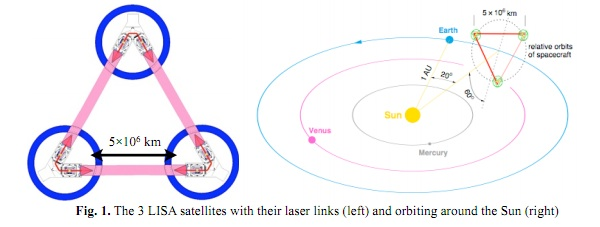
\includegraphics[width=5in]{figure1.jpg}\\\end{center}
These interferometric measurements are used to precisely monitor the distance between the inertial masses and hence to detect the tiny variation due to the passage of a gravitational wave. The goal is to detect deformations as small as $\Delta L/L\approx 7\times 10^{-21} /\sqrt{\text{Hz}}$, or 7 pm per million of km [2].

Clearly an essential technical challenge to overcome, among many others, is an outstanding precision of the phase shift measurement. Contrary to a classical Michelson interferometer, the optical signal is obtained from two different laser sources and hence the beam phase noise does not vanish and the relative frequency stability of the lasers must be at the same level as the expected sensitivity. This extreme level of stability can be achieved for LISA with three successive stabilization stages:
\begin{itemize}
\item{\bf{Time Delay Interferometry:}} Each optical signal is the combination of two laser sources, and the frequency noise of each source is also propagating on two laser links. Therefore by correctly combining the interferometric signals, taking into account the propagation delays ($\sim$ 16.7 s), it is possible to cancel the laser noises and recover a ``Michelson-like" signal. However, due to the drifts of the ultra stable clocks, this method is not perfect and the noise reduction factor is of the order of $10^8$ [2].
\item{\bf{Arm-locking:}} In the frequency range of LISA, the distance between the free-falling masses is very stable and can thus be used as a frequency reference. However, this technique relies on the frequency reference of the pre-stabilization (see below) to be slightly tunable [2].
\item{\bf{Pre-stabilization:}} Even with the above stabilization stages, the light emitted by the laser source still needs to be very stable, at the level of $10^{-13}$ relative frequency change. The foreseen technique is based on a Fabry-Perot cavity; however, another technique being developed at the APC is based on molecular iodine as a frequency reference [2,3].
\end{itemize}

We see that LISA's ability to measure very small displacements relies on accurate processing algorithms (TDI), precise feedback loops (arm-locking), and very low noise instruments (pre-stabilization). Simulation software can simulate Doppler effects, propagation delays, and the proposed algorithms for laser stabilization. However, the development of hardware detectors is desirable to characterize the detection devices, validate the numerical models, and study the influence of the hardware on the detection algorithm. This is the motivation for the LOT (LISA On Table) experiment developed at the APC.

\section{Design of the Experiment}

\indent\indent The experiment scheme is depicted in Figure 2.\\
\begin{center}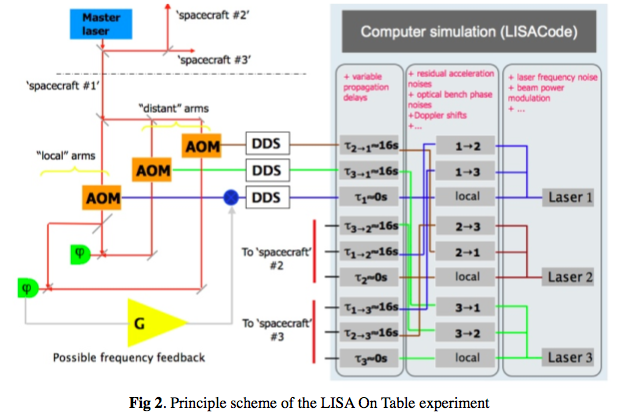
\includegraphics[width=4in]{principle.png}\\\end{center} The master laser is split to enter three different modules, each representing a LISA satellite. In each module, the beam is split again into one ``local" and two ``distant" beams. Each of these beams is given adequate frequency noise from acousto-optic modulators (AOM), which are driven by direct digital synthesizers (DDS). Each DDS generates RF signals whose frequencies, phase, and amplitude are calculated and transmitted from the computer simulation LISACode. Also developed at the APC, LISACode is a simulation software that can efficiently simulate Doppler effects, propagation delays, reconstruction algorithms, etc., which allows LOT to stay as close as possible to the real design of LISA. After the noise is added from the AOMs, two beat notes are recorded for the mixing of the local beam with each of the two distant beams [2].


%\begin{wrapfigure}[12]{r}[34pt]{1.5in}
%\centering 
%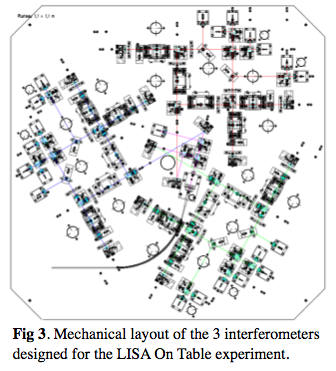
\includegraphics[width=1.5in]{mechaniclayout.png}------ stupid fucking thing
%\end{wrapfigure}


There are currently two modules mounted on the aluminum plate and for this project only one module was used. We also only used one distant arm and thus only recorded one beat note per simulation. A mechanical layout is shown below.


%EDIT TO PUT IN PIC WITHOUT PIPES
\begin{center}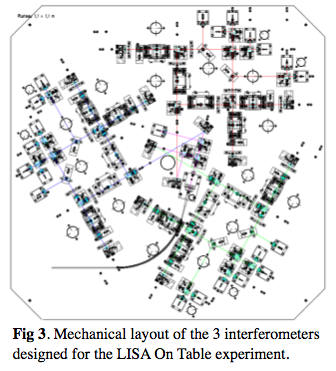
\includegraphics[width=3in]{mechaniclayout.png}\end{center}

Each module is essentially a Mach-Zehnder interferometer, with AOMs used for frequency shifting. They are arranged in "cat's eye configuration," which allows  the frequency of the laser to range over 20MHz with very little angular deviation.The DDSs drive the AOMs with a 110MHz RF signal, and due to the double pass of this configuration, the resulting frequency shift of the beam is 220MHz. The use of AOMs also allows the two distant arms to travel on the same optical path, but with perpendicular polarizations [2].

The set up very precisely ensures that each laser beam propagates with exactly the same optical path and components. Below 1 Hz, the predominant phase disturbances are due to thermal dilation of the bench. However, since the optical paths are identical, the phase is insensitive to the isotropic dilation due to homogenous temperature variations. In the future it is possible that the experiment may be mounted on Invar plates. The objective of this project is to determine the correlation between non-homogeneous temperature variation and phase noise.


\section{Correlating Noise with Temperature Variation}

\indent\indent We begin by placing platinum plated resistors along the arms of one module mounted on the aluminum plate to record temperature.\\\begin{center}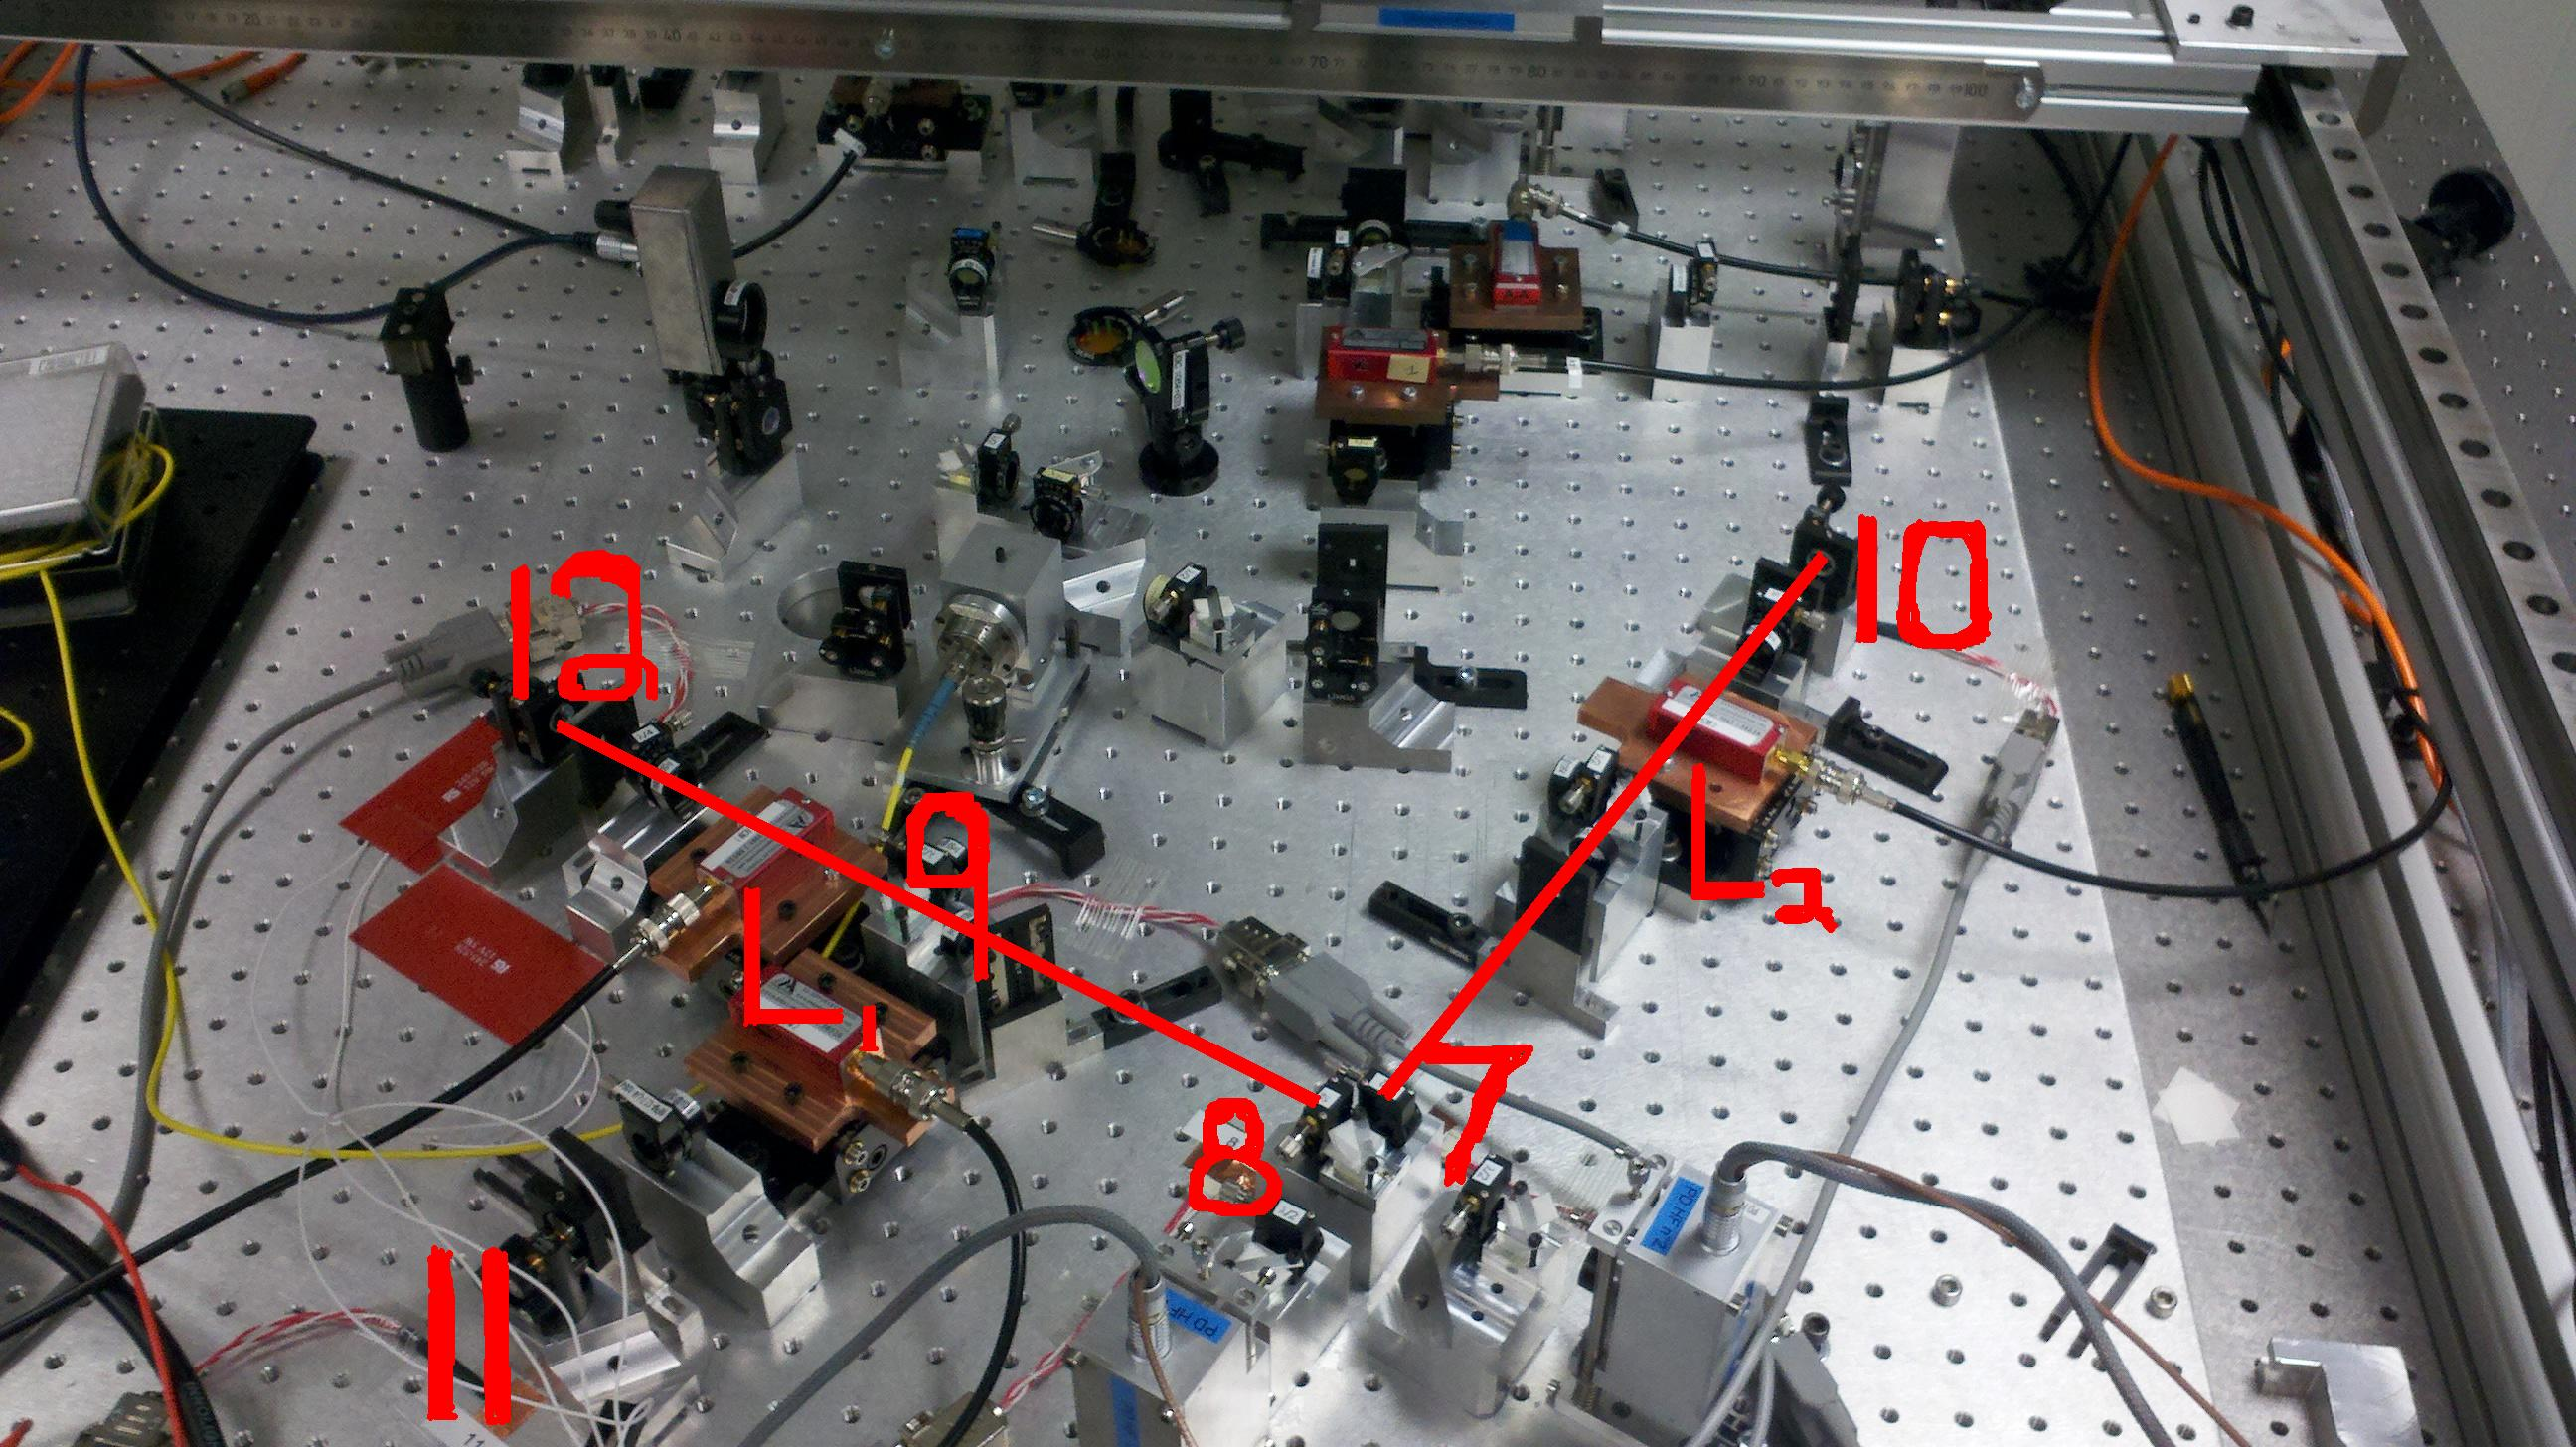
\includegraphics[width=5.5in]{expectations.jpg}\end{center}

There are six temperature sensors labeled 7 through 12 to be consistent with the channels used on the National Instruments control panel. We expect that thermal expansion affecting arm $L_1$ will be caused by variation between $\{T_9, T_{11}, T_{12}\}$ and $\{T_7,T_8\}$, while variation between  $T_{10}$ and $\{T_7,T_8\}$ will affect arm $L_2$, such that 
$$\delta L_1 \propto \left\{\begin{array}{l} T_9 \\T_{11} \\T_{12}\end{array}\right. - \left\{\begin{array}{l} T_7 \\T_8 \end{array}\right.\hspace{.5cm}\text{and}\hspace{.5cm} \delta L_2 \propto T_{10} - \left\{\begin{array}{l} T_7 \\T_8 \end{array}\right..$$ We expect that there will be more noise if one arm has much greater variation than the other, such that the phase noise will be proportional to the difference between the small change in each length: $$\delta\varphi\propto\delta L_1-\delta L_2.$$

We let the simulator run over night and recorded the temperature and phase in LabVIEW. Then using Python, we extracted the temperature and phase data shown below.

\noindent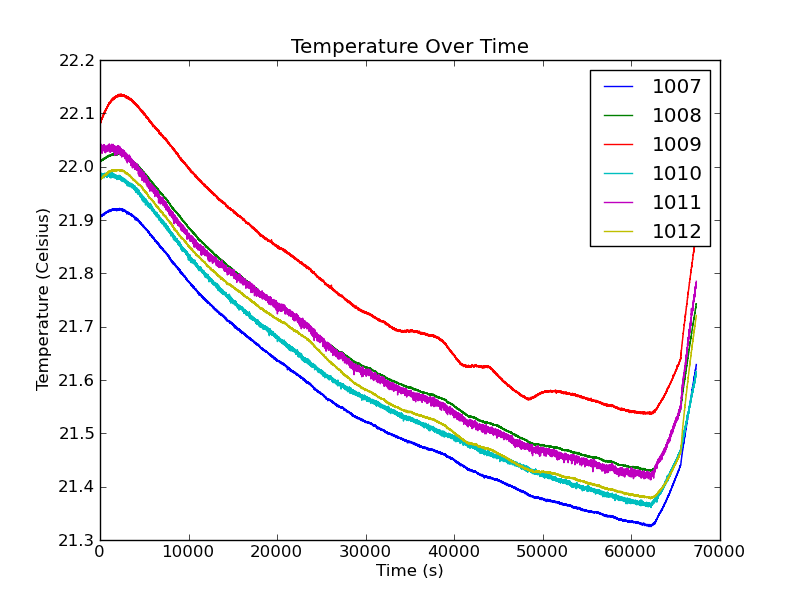
\includegraphics[width=3.2in]{Figure2.png}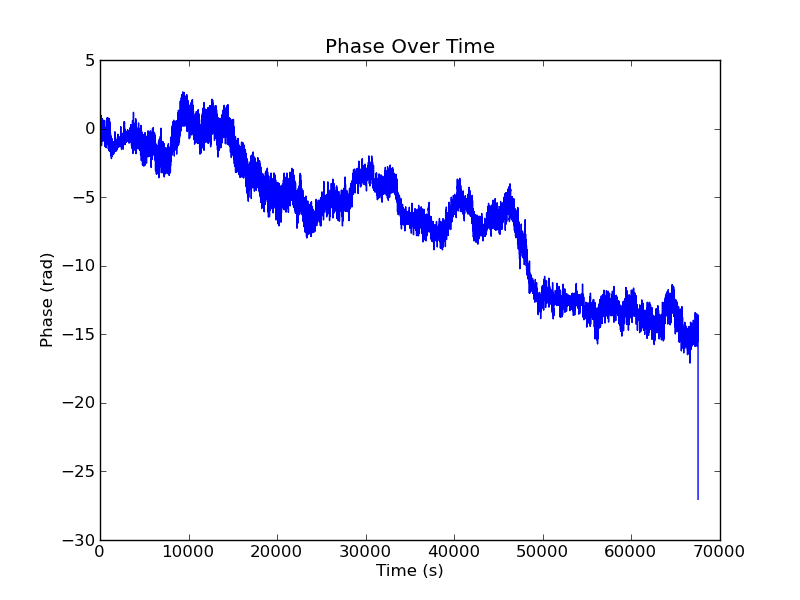
\includegraphics[width=3.2in]{Figure3.png}\vspace{.7cm}
While the global temperature changed over time, the variation is not too great among the seven channels. We see that $T_9$ seems to have the greatest variation from the rest of the channels, from around $3\cdot 10^4$ s to $5\cdot 10^4$ s. If the variation between $T_{10}$ and $\{T_7,T_8\}$ is small relative to the variation between $T_9$ and $\{T_7,T_8\}$, this will correspond variation of $L_1$ being greater than that of $L_2$. We hope that this will correspond to the phase noise. We graph $T_9-T_7$ and $T_{10}-T_7$ after subtracting the respective means of each difference.

\begin{center}\noindent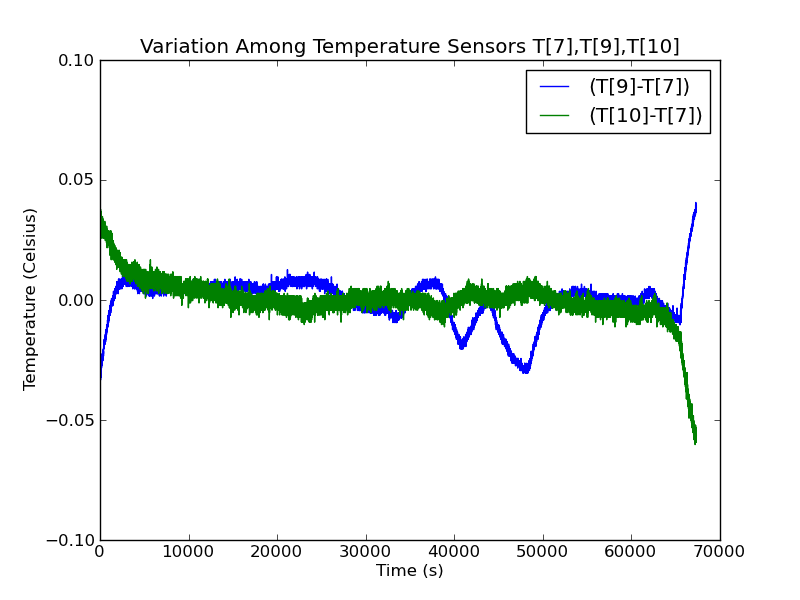
\includegraphics[width=3.2in]{Tempdiff_7-9-10.png}\\\end{center}
We can see that there is indeed very little variation along $L_2$ and somewhat greater variation along $L_1$. We now attempt to correlate this variation with phase noise.
Again in python, we obtain a normalized cross spectral density between the phase and the difference $T_9-T_7$. Python uses Welch's average periodogram method to compute the CSD. The command has a parameter called NFFT, which is the number of data points used in each block for the Fast Fourier Transforms (FFT). In computing our CSDs, we must make a decision of how long each block will be; the higher the NFFT, the more frequency resolution the graph will have, but it will also be more susceptible to noise. Any noise in the graph should be directly proportional to the NFFT parameter. These normalized CSDs were computed as $$CSD_N(f)=\frac{|CSD(phase, T_9-T_7)|} { \sqrt{PSD(phase)\cdot PSD(T_9-T_7)}}.$$
\begin{center}\noindent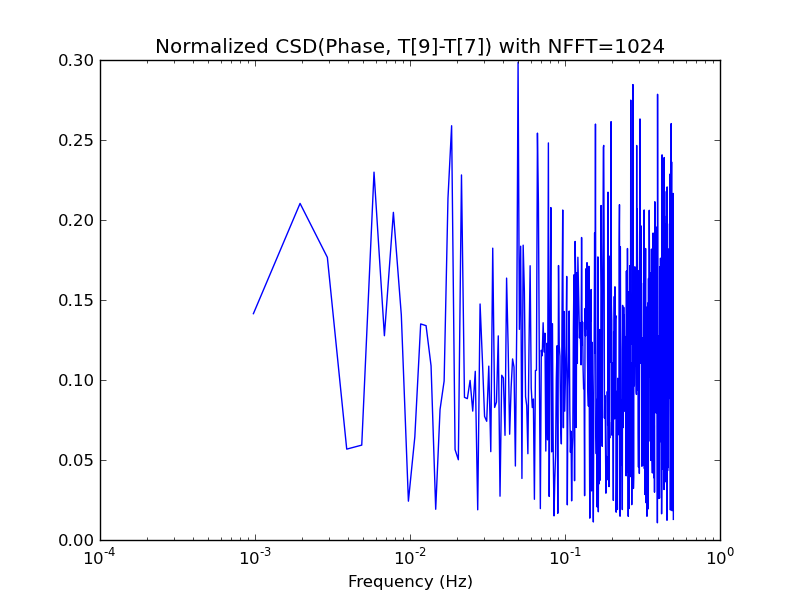
\includegraphics[width=3in]{CSDNFFT1024.png}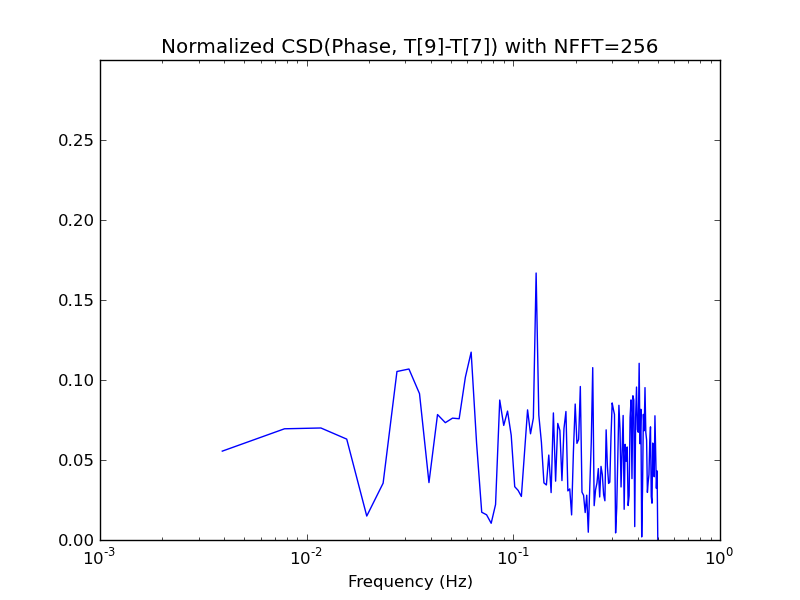
\includegraphics[width=3in]{CSDNFFT256.png}\end{center}
The graph above to the left was computed with NFFT = 1024, and we already see that there is very low correlation, with no strong signal anywhere in the frequency band. The way our normalized CSD was computed will yield a maximum of 1 when the two signals are at perfect correlation for a given frequency, while 0 corresponds to no correlation. To ascertain this, to the right we have the CSD computed at NFFT = 256, and we see that the little correlation we had drops lower, and we are simply seeing noise here. In the next section we employ more sophisticated methods to find the desired correlation.


\section{Lessened Air Turbulence and Modulated Temperature}

\indent\indent Air turbulence is predicted to be one of the largest sources of noise for this experiment. In the end, LOT will be modified for a vacuum chamber, but until then we will have the noise associated with air in the clean room. The noise from the air turbulence may have been masking the noise from temperature variation, so we might be able to find a correlation if we can shield the beam from turbulence. To do this, we cut appropriately sized PVC pipe and built simple adjustable stands for the pipes. We then lined them along the arms of the module, such that the beam goes through the pipe and is better shielded from turbulence.\\\begin{center}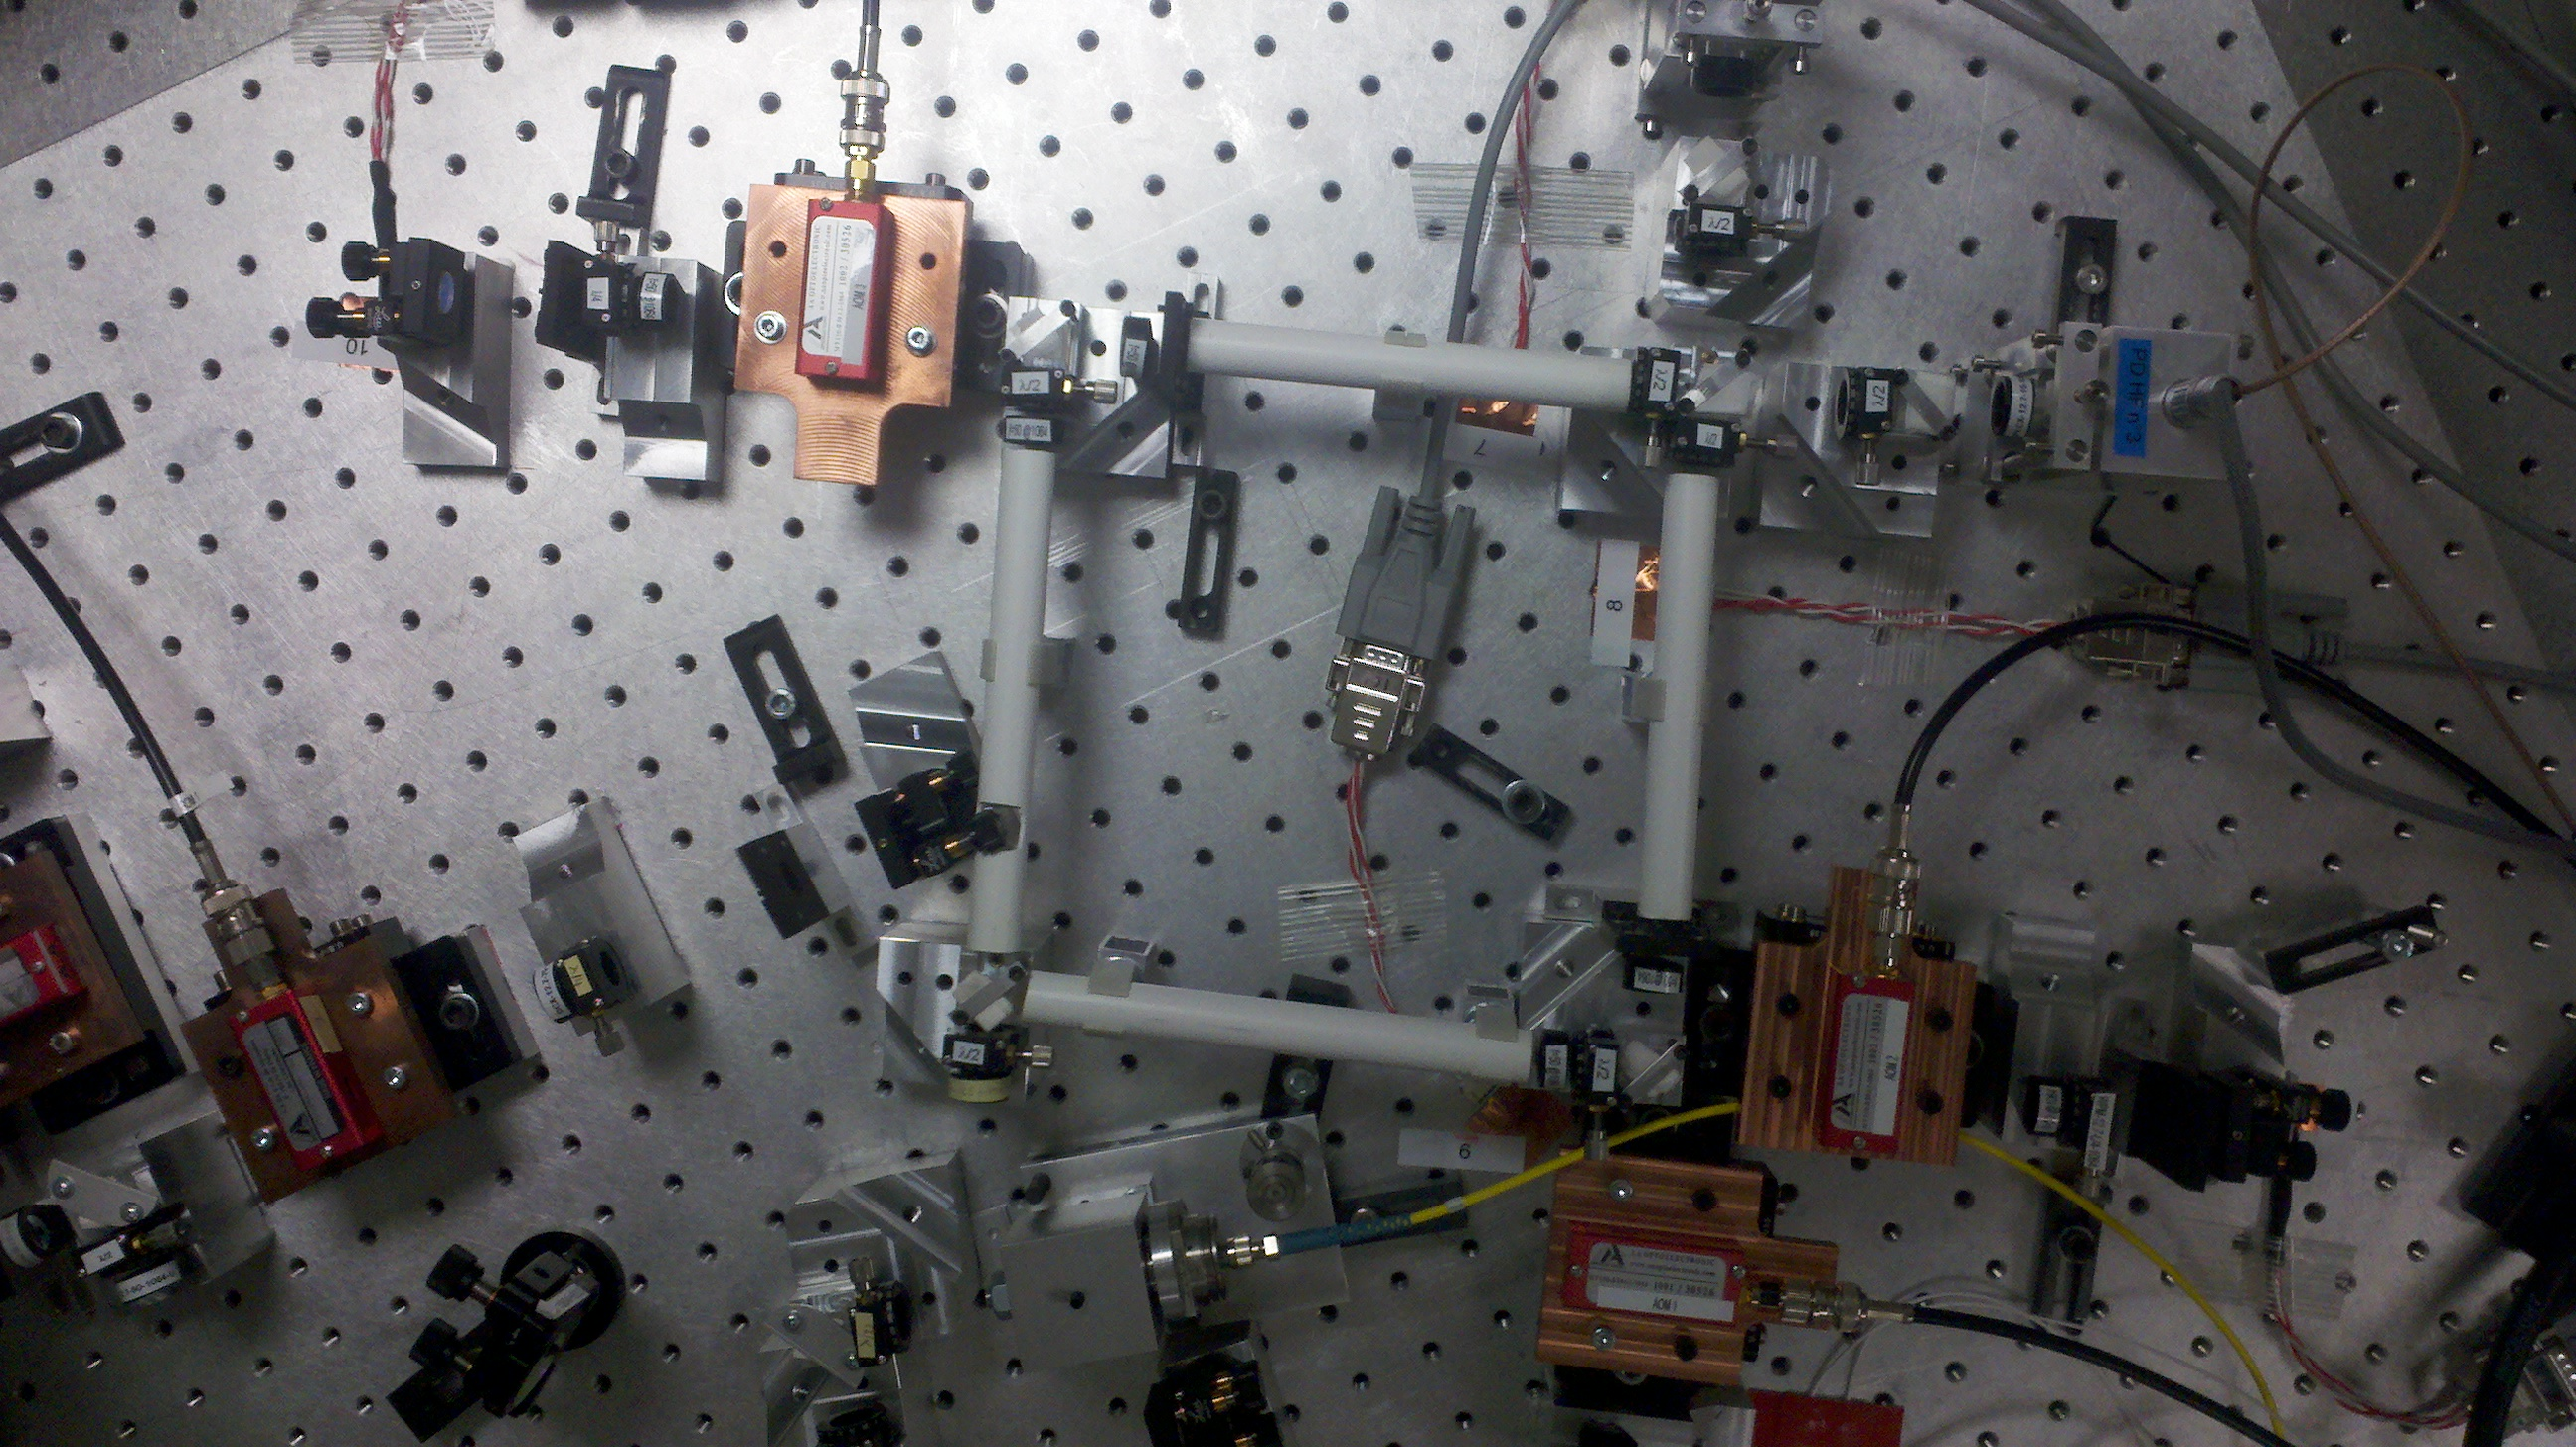
\includegraphics[width=4.5in]{piping.jpg}\\\end{center} Not every part of the beam is shielded, as our stands would not fit in certain sections near the AOMs. However, the pipes do surround the beam on the long sections along the arms where there are not many components- which is probably where most of the turbulence affects the beam.

It will also be much easier to find a correlation with temperature if we control and increase the temperature fluctuation on the bench. We leave arm $L_2$ alone, and put down 12V heating pads at the end of arm $L_1$.\begin{center} 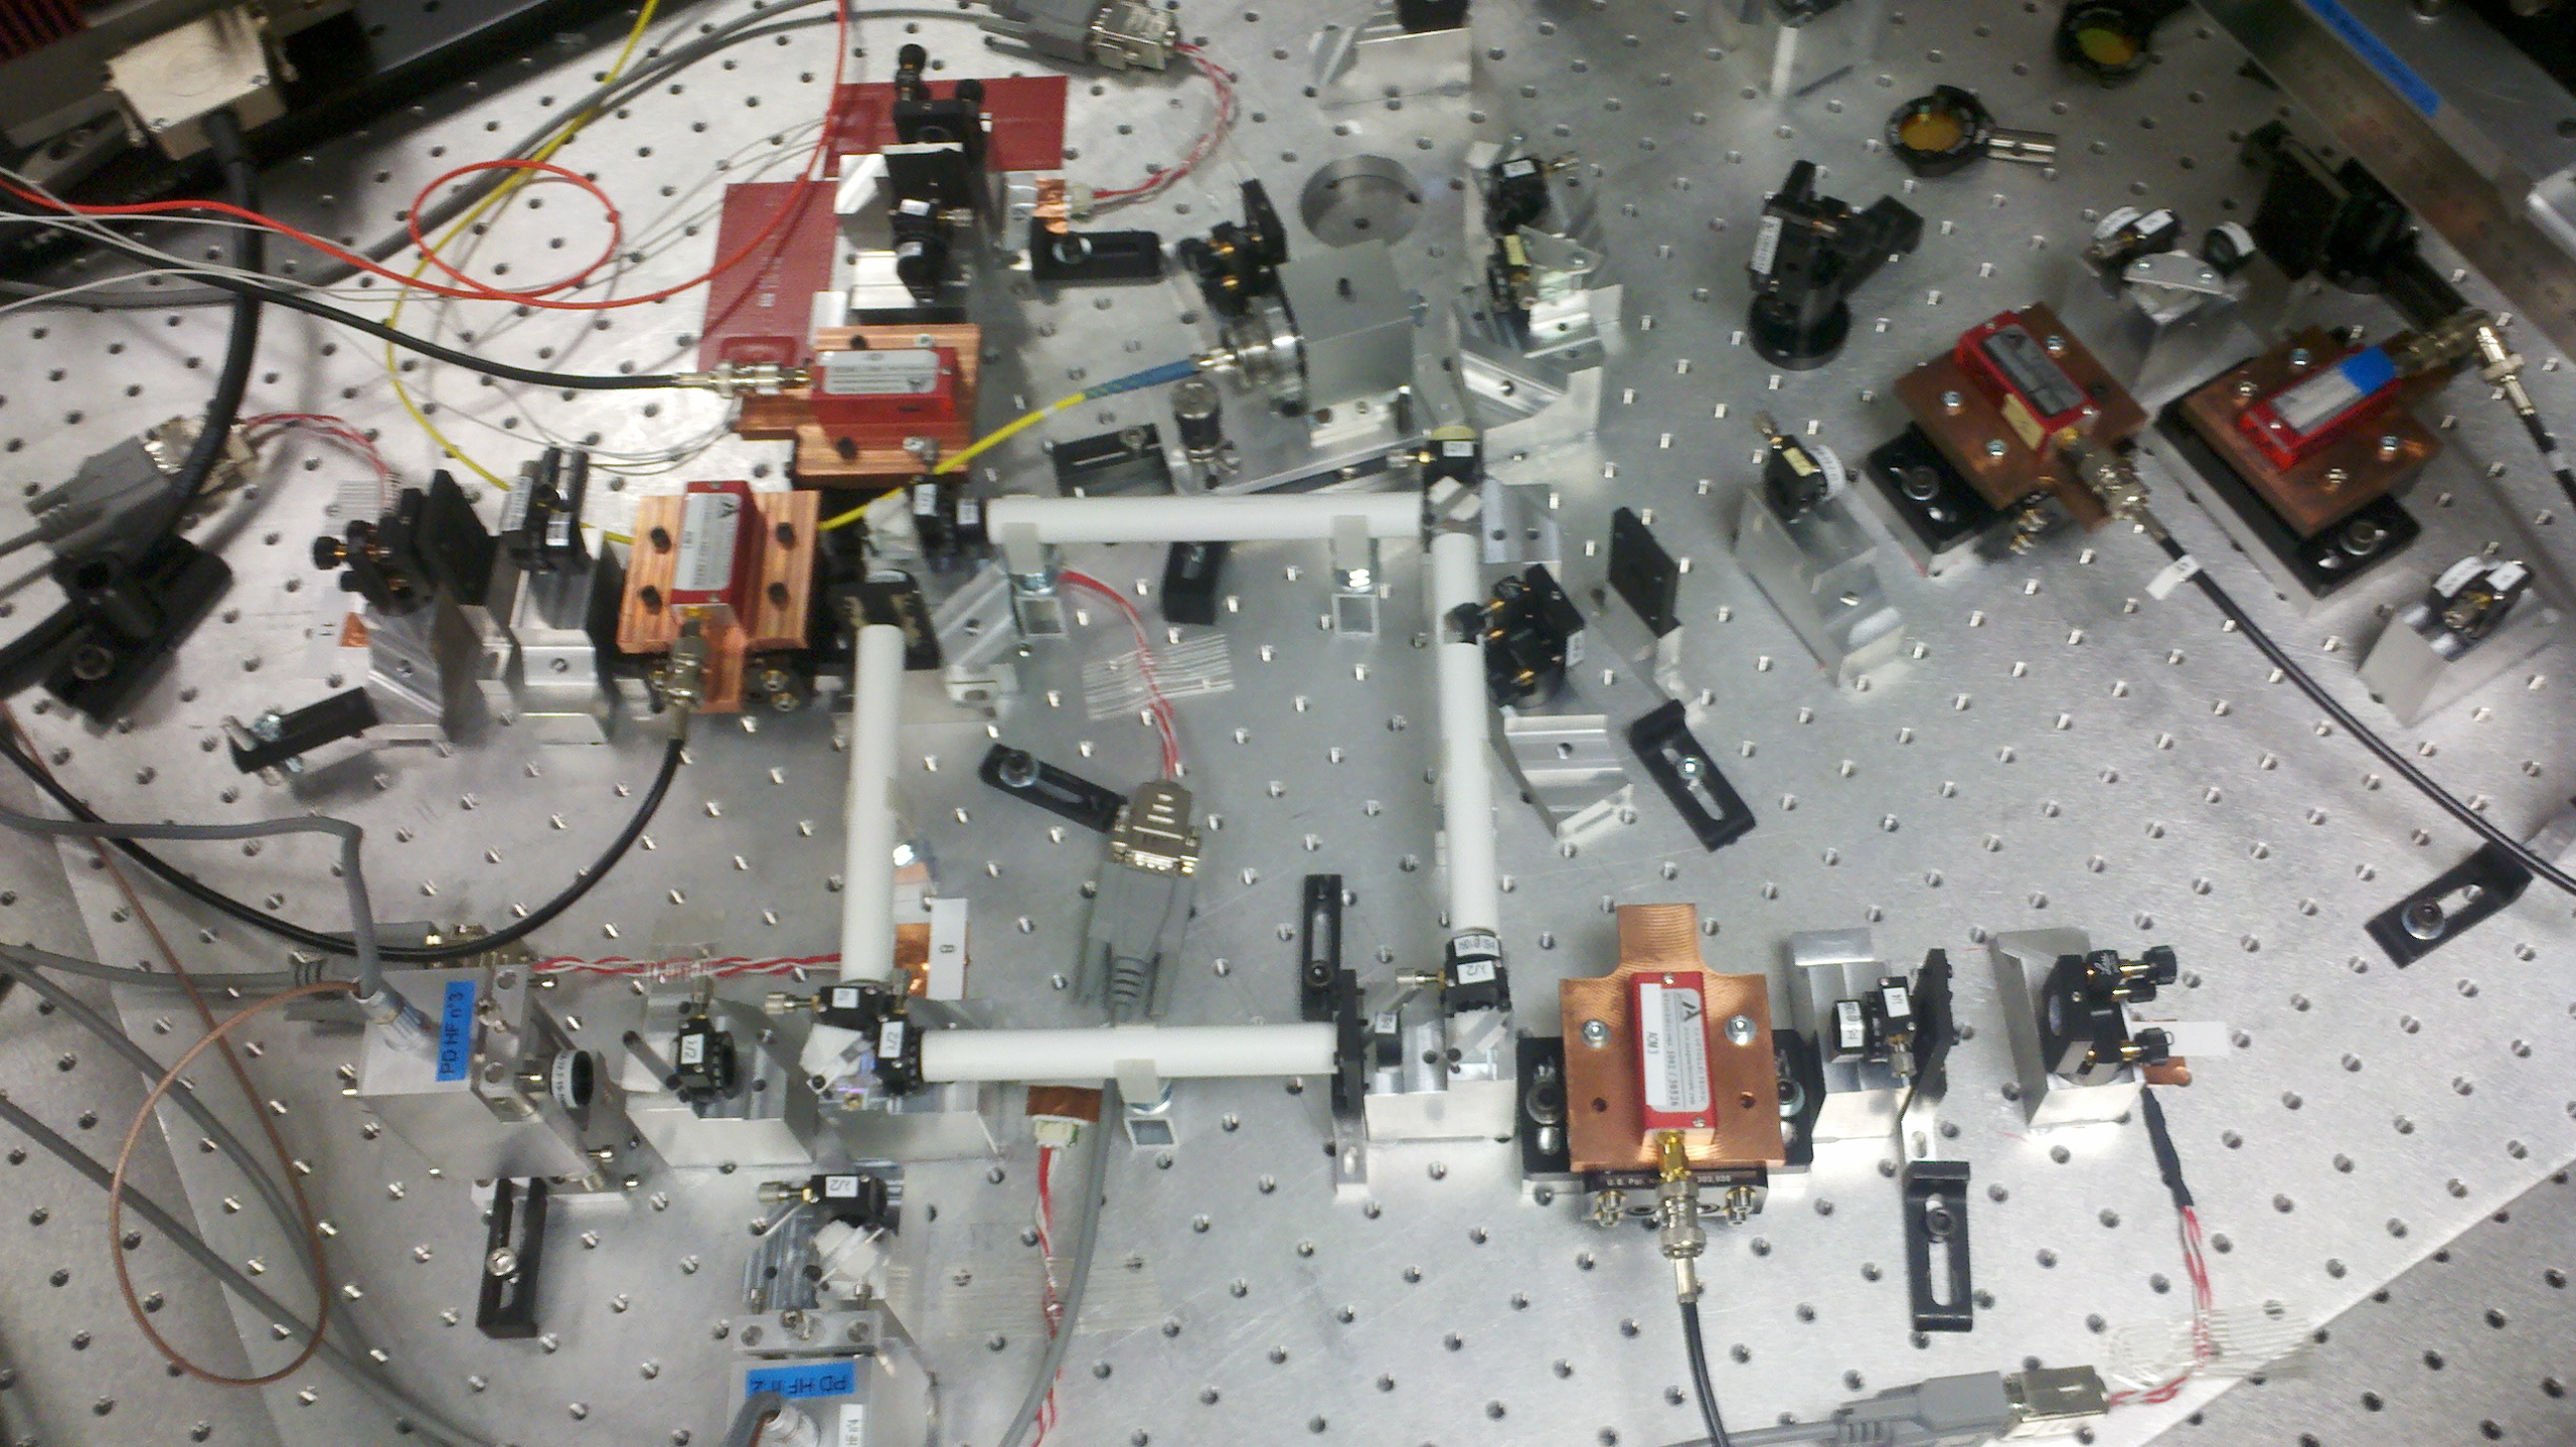
\includegraphics[width=4in]{heatingpads.jpg}\\\end{center}The heating pads are wired to a function generator that is controlled by the same LabVIEW program that we use to record the temperature. We set the pads to modulate at an offset of 6V with an amplitude of 6V at 1mHz. So the voltage applied will vary from 0 to 12V in cycles of 1000s, approximately 17 minutes.

\section{Results}
\indent\indent Again we let the simulator run over night and obtained temperature and phase data through LabVIEW, shown below.
\begin{flushleft}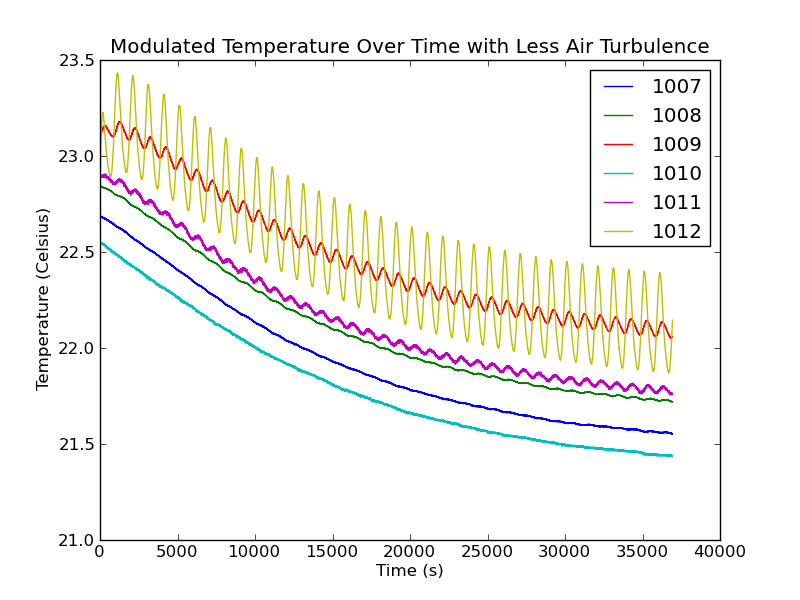
\includegraphics[width=3.1in]{ModulatedTemp.png}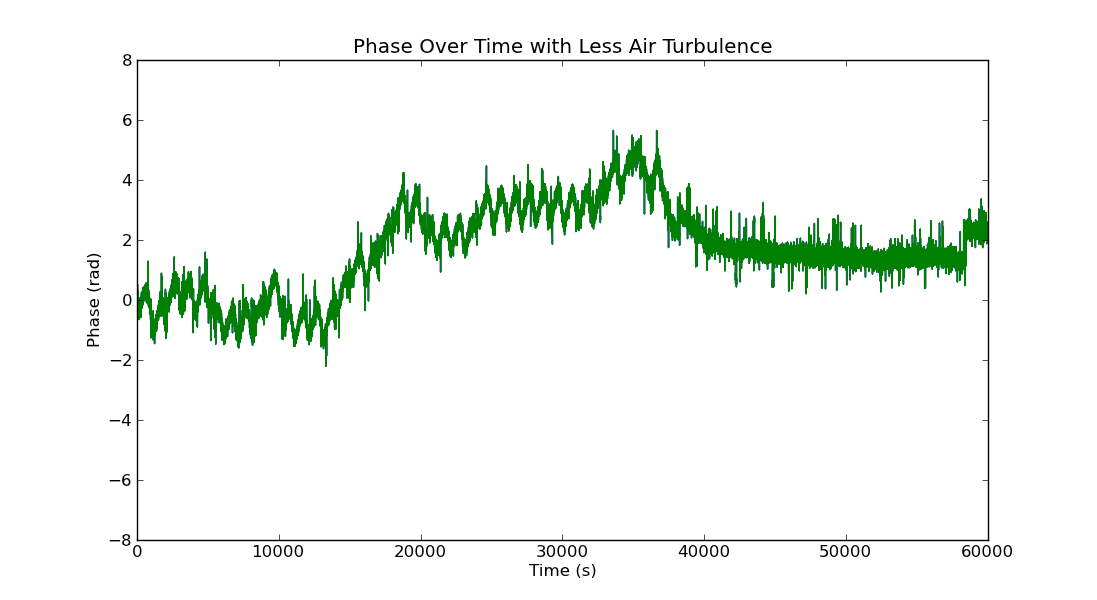
\includegraphics[width=4.1in]{phase260711.png}\\\end{flushleft}

Now we see a very clear and clean variation between $\{T_{9},T_{11},T_{12}\}$ and the rest of the temperature sensors. We also note that the temperature variation along $L_2$ is very minimal compared to $L_1$, as shown in the image below to the left. A quick look at the time scales of the above two graphs reveals that the LabVIEW program controlling the temperature modulation and recording crashed about halfway through the data acquisition, a little after $3.5\cdot 10^4$ s. We see in the phase graph that there is clearly an oscillation in the phase up until this time, which leads us to believe we have found the correlation.
We now compute the PSD of the variation between $T_{12}$ and $T_7$. Although there is also fluctuation of $T_{11}$ and $T_9$, we will use $T_{12}$ because the variation is more pronounced. We compute the PSD of the temperature difference $T_{12}-T_{7}$ in python, with NFFT sampling at 8192, shown below to the right.
\begin{center}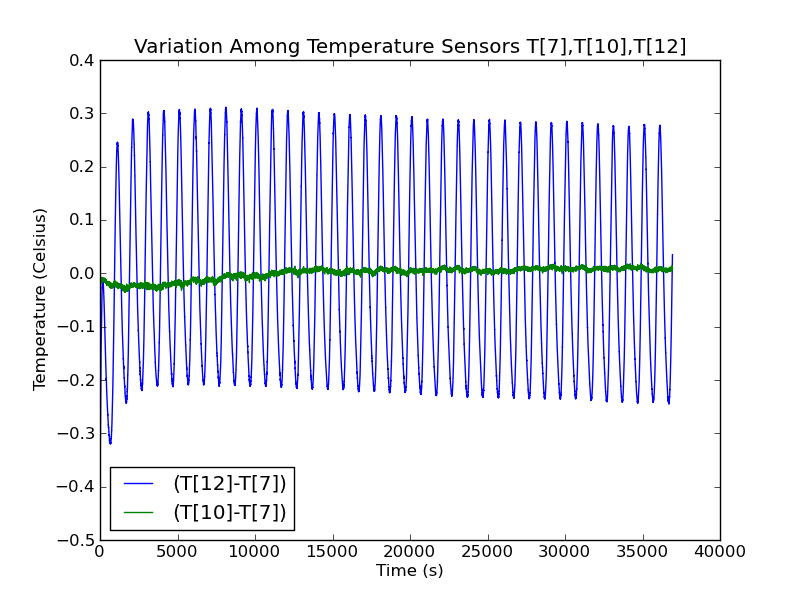
\includegraphics[width=3in]{Tempmoddiff_7-10-12.png}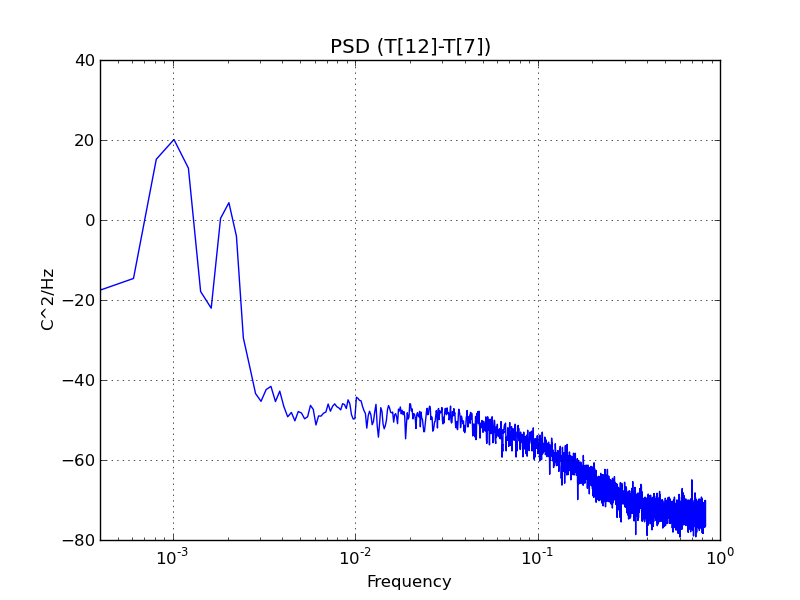
\includegraphics[width=3in]{PSD_mod12-7.png}\\\end{center} As we expected to find, there is a very distinct peak at 1 mHz. There is also a well defined peak at 2 mHz, which is most likely the first harmonic of this oscillation. Next we plot the PSD of the phase (using only the data up to $3.5\cdot 10^4$ s) with the same NFFT parameter, shown below.
\begin{center}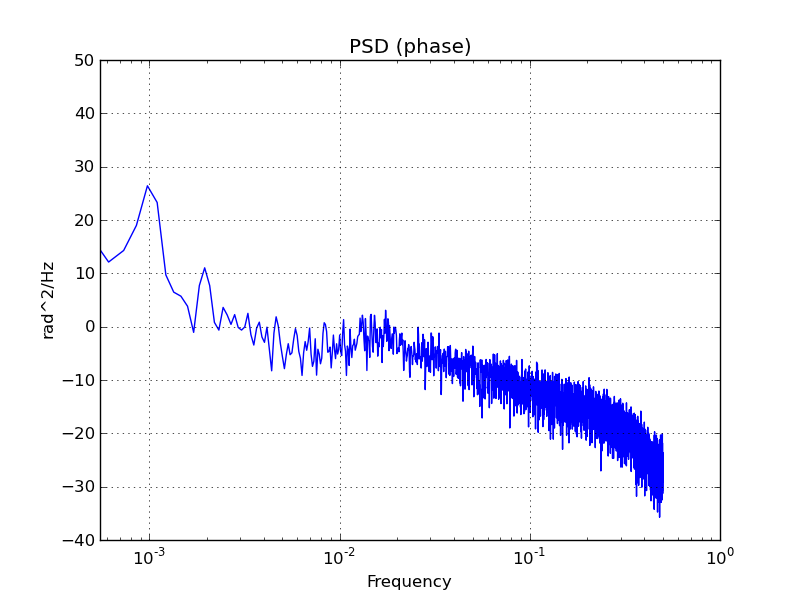
\includegraphics[width=4in]{PSD_phasemod.png}\\\end{center}
With this PSD, we can immediately see that there is a true correlation between non-homogenous temperature variation and phase noise. There is a very distinct peak at 1 mHz and again the smaller peak around 2 mHz, both of which are characteristics of the temperature PSD.

Finally, to validate this correlation we compute a normalized CSD between the two sets of data. Again we only use the appropriate amount of phase data, and since for this run the sampling time for the phase is 1.0 s and the sampling time for the temperature is 0.6 s, it was also necessary to linearly interpolate the temperature to be on the same time reference as the phase. This consists of simply finding the linear relationships from one data point to the next for the temperature data (connecting the dots to make a piecewise linear function), and then using the equations to find the approximate value of the temperature at each of the discrete time values for which we have phase data points. A simple program in python can accomplish this, and then we compute the normalized $CSD_N(f)$ as in Section 3, shown below.
\begin{center}\noindent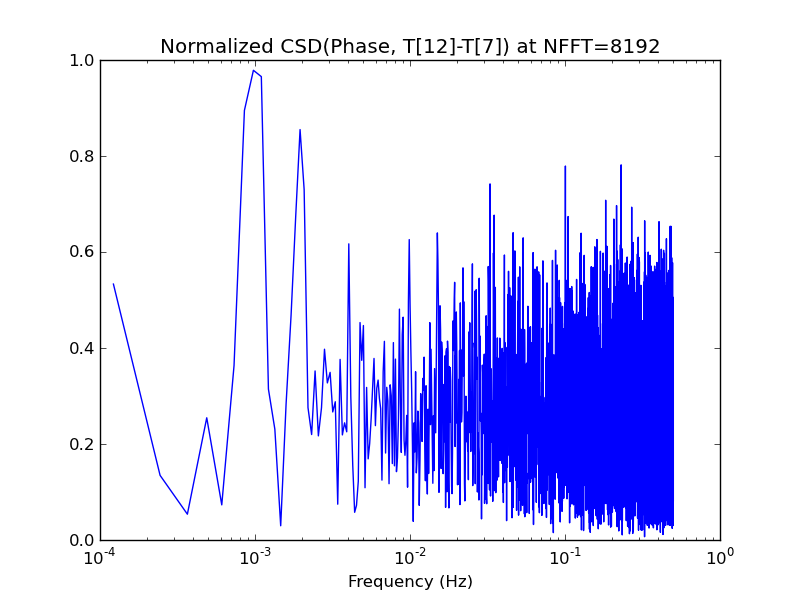
\includegraphics[width=3.5in]{CSDNFFT8192.png}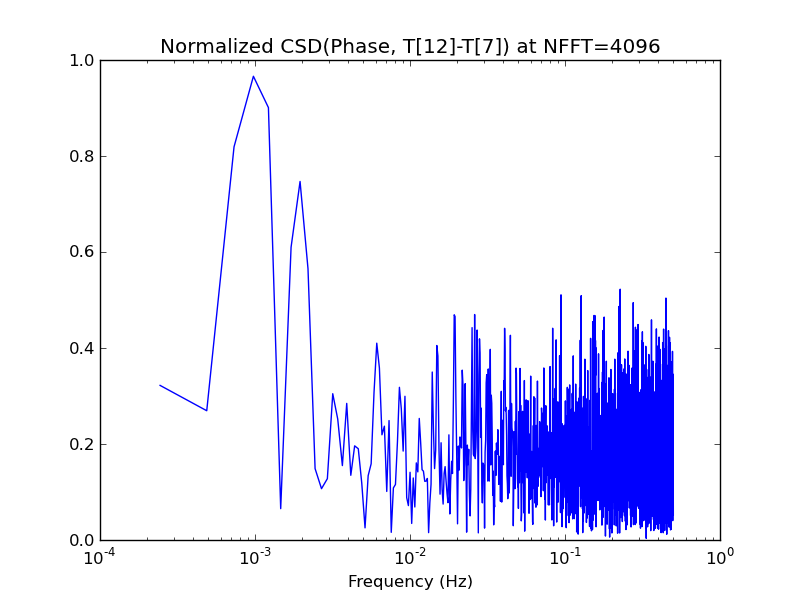
\includegraphics[width=3.5in]{CSDNFFT4096.png}\\\end{center}

As expected from looking at each PSD, we have almost a full correlation at 1 mHz. We see that as mentioned earlier, the higher frequency noise drops when we decrease the size of the FFT blocks; yet the peaks around the 1 mHz temperature modulation and first harmonic remain. Thus, we can be confident that our results are conclusive.

\section{Conclusion and Future Plans}

\indent\indent We have successfully correlated temperature variation with phase noise and will continue in this direction, analyzing the data further to find the appropriate relation. In the next few weeks we aim to find a formula for the required minimal temperature variation needed to achieve a threshold of phase noise. The results of this project are also valuable to the APC as a greater incentive to mount the simulator on an Invar plate, which is currently undecided. However, after finding the formula mentioned above we may be able to keep the sensors on the aluminum plate and use the formula to account for the temperature variation affecting recorded phase data. Although it might not seem like a ``good" result to prove that our aluminum plate is intrinsically a source of noise, it is important and worthwhile to find these results with certainty, so that we can characterize the noise.

\end{document}

%[1] is the LISA government site
%[2] is the APC optical simulator paper
%[3] is the APC stabilization paper











